% v1.3.2: exact copy of the corrected main.tex, kept as the pandoc DOCX source.
\documentclass[11pt,reqno]{amsart}

\usepackage[T1]{fontenc}
\usepackage[utf8]{inputenc}
\usepackage{amsmath,amssymb,amsthm,mathtools}
\usepackage{graphicx}
\usepackage{booktabs}
\usepackage[margin=1in]{geometry}
\usepackage[protrusion=true,expansion=false]{microtype}
\usepackage{xcolor}
\usepackage[colorlinks=true,linkcolor=blue!55!black,citecolor=green!45!black,urlcolor=blue!55!black]{hyperref}

\theoremstyle{plain}
\newtheorem{theorem}{Theorem}[section]
\newtheorem{lemma}[theorem]{Lemma}
\newtheorem{proposition}[theorem]{Proposition}
\newtheorem{corollary}[theorem]{Corollary}
\theoremstyle{definition}
\newtheorem{definition}[theorem]{Definition}
\newtheorem{remark}[theorem]{Remark}
\newtheorem{observation}[theorem]{Observation}

\DeclareMathOperator{\tr}{tr}
\DeclareMathOperator{\adj}{adj}
\DeclareMathOperator{\Hess}{Hess}
\newcommand{\R}{\mathbb{R}}
\newcommand{\C}{\mathbb{C}}
\newcommand{\Sph}{\mathbb{S}}
\newcommand{\calT}{\mathcal{T}}
\newcommand{\calD}{\mathcal{D}}
\newcommand{\Fz}{F_{z}}
\newcommand{\eps}{\varepsilon}
\newcommand{\ie}{i.e.\ }
\newcommand{\eg}{e.g.\ }

\begin{document}

\title[Exact fiber elimination for the PCR3BP convexity gates]{Exact fiber elimination for the Levi--Civita convexity gates of the planar restricted three-body problem, with a global convexity reconnaissance}

\author{C\'esar Augusto Grisa}
\address{Instituto de Computa\c{c}\~ao, Universidade Federal Fluminense, Niter\'oi, RJ, Brazil}
\email{cagrisa@id.uff.br}

\date{\today}

\subjclass[2020]{Primary 70F07; Secondary 37J06, 53A07, 68W30}
\keywords{Restricted three-body problem, Levi--Civita regularization, strict convexity, global surface of section, Birkhoff conjecture, computer-assisted proof}

\begin{abstract}
Computer-assisted strict-convexity certification of the regularized energy surfaces of the planar circular restricted three-body problem (PCR3BP) reduces to the simultaneous positivity of two scalar \emph{gates}, $T$ and $D$, over a four-dimensional domain: a two-dimensional Levi--Civita base times a fiber angle $\phi\in\Sph^1$. We prove four exact algebraic identities that eliminate the fiber angle in closed form. The tangential gate satisfies $\min_\phi T = \calT$ with $\calT$ an explicit function of the base alone, attained at a computable angle; the curvature-determinant gate admits an exact five-term harmonic decomposition whose second-harmonic amplitude is $128F^2 s$ for the structure matrices at hand, yielding the rigorous lower bound $D\ge \calD := A_0-\sqrt{A_1^2+B_1^2}-128F^2 s$, which is sharp on the collar. Both gates thereby reduce from four variables to two, unconditionally. All identities are confirmed by an exact symbolic audit whose residuals vanish identically. As an application, the reduced gates reproduce the certified convexity bounds near the Earth--Moon mass ratio (the regularized component being the Moon's). Using the reduced gates we compute a global reconnaissance of Levi--Civita convexity across the mass--energy plane, parametrized by the mass fraction $m_r$ of the regularized primary. Near the critical energy the non-convex window is large and asymmetric: at $\Delta c=10^{-4}$ it spans $m_r$ from $\approx 0.045$ to beyond $0.999$, so only components regularized at a sufficiently light primary are LC-convex there. This is consistent with Kim's near-critical non-convexity theorem for the heavy-primary component below the $16/17$ mass fraction, and shows that his sufficient condition is far from sharp near the critical energy: the heavy-side non-convexity persists essentially up to the rotating-Kepler limit. We record a numerical observation that the non-convexity region avoids the collision-orbit axes and forms lateral lobes on which the failure is a single simple fold---one negative principal curvature, the tangential gate staying positive---while the base remains radially star-shaped; and we delimit the (provably open) comparable-mass regime. A refinement of the reconnaissance down to energy offsets of $10^{-7}$ reveals that even the Moon component of the Earth--Moon system ($m_r\approx 0.0122$) loses LC-convexity on an ultrathin shell of width $\approx 9.5\times 10^{-6}$ above the critical energy, where the Lagrange point enters the surface; the Earth component ($m_r\approx 0.9878$) is non-convex on a macroscopic near-critical window, recovering LC-convexity only for $\Delta c\gtrsim 1.2\times 10^{-2}$. This locates the natural boundary of the LC route at the critical limit. (This is version~2 of the paper: it corrects a mass-convention mislabeling and a scanning-heuristic flaw of version~1; see the erratum note in Section~\ref{sec:map}.)
\end{abstract}

\maketitle

\section{Introduction}\label{sec:intro}

\subsection{Background}
Let $\mu\in(0,1)$ be the mass ratio of the two primaries of the planar circular restricted three-body problem (PCR3BP). For energies below the first critical Jacobi value the regularized bounded components of the energy hypersurface are diffeomorphic to $\Sph^3$ and are known to be star-shaped~\cite{AFKP}. A central structural question, going back to Birkhoff~\cite{Birkhoff}, is whether the retrograde periodic orbit on each bounded component bounds a disk-like global surface of section. By the theorem of Hofer, Wysocki and Zehnder~\cite{HWZ}, a closed \emph{strictly convex} hypersurface in $\R^4$ carries such a section; and by the refinement of Hryniewicz and Salom\~ao~\cite{HS}, dynamical convexity of a regularized $\Sph^3$ suffices to produce a rational open book whose binding is a distinguished periodic orbit and whose pages are global surfaces of section. Establishing strict convexity of the regularized surface is therefore a concrete and sufficient route towards the Birkhoff conjecture for a given parameter regime.

The standard double cover is the Levi--Civita (LC) regularization~\cite{LeviCivita}, which sends the regularized bounded component to a compact hypersurface $\Sigma_{\mu,c}=\{K_c=0\}\subset\R^4\cong\C^2$. Whether the LC embedding is convex is a delicate matter. Kim~\cite[Thm.~1.3]{Kim} proved that the LC image of the regularized heavy-primary component fails to be convex for energies close to the critical value once the heavy-primary mass fraction drops below $16/17$; the same paper~\cite[Thm.~1.1]{Kim} shows that the doubly-covered elliptic (two-center) coordinates furnish a genuinely convex embedding for the Euler problem, and, switching on the rotation term, establishes the analogous convexity for the rotating problem only in the perturbative regime of small rotation strength~\cite[Rmk.~1.2]{Kim}, leaving the full PCR3BP as the stated goal. Thus the LC-convexity route is powerful but has a known ceiling in the comparable-mass, near-critical corner of parameter space.

\subsection{The computational bottleneck}
A computer-assisted convexity certificate on a fixed parameter box proceeds by verifying, with interval arithmetic, that a pair of scalar \emph{gates} $T$ and $D$ are strictly positive at every point of the regularized surface~\cite{GrisaCertificate}. After the LC reduction the surface fibers over a compact two-dimensional base $z=(z_1,z_2)$ by an angle $\phi\in\Sph^1$, so each gate is a function of the four real variables $(z_1,z_2,\phi)$ (with the parameters $\mu,c$ fixed). The angular variable multiplies the cost of certification: every base cell must be checked against the whole circle of fiber directions, and the interval enclosures of trigonometric expressions inflate the bounds. Eliminating $\phi$ analytically---replacing the four-dimensional gate by a sharp two-dimensional surrogate---removes this fiber sweep entirely.

\subsection{Contributions}
This paper makes the following contributions.
\begin{enumerate}
\item[(i)] \textbf{Exact fiber elimination.} We prove four algebraic identities (Lemmas~\ref{lem:T}--\ref{lem:amp}) that reduce both gates from the four variables $(z,\phi)$ to the two base variables $z$. For the tangential gate the reduction is an exact minimum, $\min_\phi T=\calT(z)$, attained at an explicit angle. For the curvature-determinant gate we obtain an exact harmonic decomposition and a rigorous, collar-sharp lower bound $D\ge\calD(z)$. Section~\ref{sec:elimination}.
\item[(ii)] \textbf{Symbolic certification.} Every identity is confirmed by an exact computer-algebra audit whose eight residuals vanish identically; the audit is short, deterministic, and included in the reproducibility package (Appendix~\ref{app:audit}).
\item[(iii)] \textbf{Application.} The reduced gates reproduce the certified strict-convexity bounds near the Earth--Moon mass ratio (Section~\ref{sec:earthmoon}).
\item[(iv)] \textbf{Global reconnaissance.} Using the reduced gates we compute a floating-point map of LC-convexity across the mass--energy plane, in the mass fraction $m_r$ of the regularized primary. Near the critical energy the non-convex window spans $m_r\in(\approx 0.045,\,>0.999)$, consistent with (and extending well beyond) Kim's $16/17$ sufficient condition for the heavy-primary component; the window closes for $\Delta c\gtrsim 0.03$ at every mass ratio scanned (Section~\ref{sec:map}).
\item[(v)] \textbf{A dynamical-relevance observation.} We record numerical evidence that the non-convexity region avoids the collision-orbit axes and that, on the lateral lobes where it lives, the failure is a single simple fold on a base that stays radially star-shaped; and we discuss the provably open comparable-mass regime (Sections~\ref{sec:relevance}--\ref{sec:outlook}).
\end{enumerate}
Contributions (i)--(ii) are rigorous; (iii) is a reproduction of an existing certified computation; (iv)--(v) are floating-point reconnaissance and are labeled as such throughout.

\section{The regularized surface and the convexity gates}\label{sec:setup}

\subsection{Levi--Civita coordinates}
In the barycentric rotating frame, place the primaries on the $q_1$-axis and pass to Levi--Civita coordinates $z=(z_1,z_2)\in\R^2$ via $q=2\bar z^2$. Writing $s=|z|^2=z_1^2+z_2^2$ and $a=z_1^2-z_2^2$, the regularized defining function for the bounded component takes the form
\begin{equation}\label{eq:F}
F(z)=1-\mu+\frac{2\mu s}{\sqrt{1-4a+4s^2}}-2cs+\mu^2 s+4s^3-4\mu s a,
\end{equation}
where $c$ is one half of the Jacobi constant. The regularized surface is $\Sigma_{\mu,c}=\{F=0\}$ in the appropriate sense; the locus $\{F=0\}$ is the \emph{collar} in the base. Note that $F$ depends on $z$ only through the pair $(s,a)$; this is used repeatedly below.

\begin{remark}[Mass convention]\label{rem:mass}
In~\eqref{eq:F} the parameter $\mu$ is the mass fraction of the \emph{distant} primary, located at $q=(1,0)$; the \emph{regularized} primary, at the origin, has mass fraction $m_r=1-\mu$. Indeed, writing $\Omega(q)=\tfrac12|q-b|^2+(1-\mu)/|q|+\mu/|q-e|$ for the effective potential of the pair with mass $1-\mu$ at the origin, mass $\mu$ at $e=(1,0)$ and barycentre $b=(\mu,0)$, the substitution $q=2\bar z^2$ gives the exact identity $F=|q|\,(\Omega(q)-c)$, reproducing~\eqref{eq:F} term by term ($\sqrt{1-4a+4s^2}=|q-e|$, $\mu^2 s=\tfrac12\mu^2|q|$ from the barycentric offset, $-4\mu sa=-\mu q_1|q|$); the identity is verified symbolically in the reproducibility package. Version~1 of this paper mislabeled $m_r$ as $\mu$ itself in the reconnaissance sections; all component attributions below use the corrected convention.
\end{remark}

\subsection{The two gates}\label{sec:gates}
Certifying that $\Sigma_{\mu,c}$ bounds a strictly convex domain reduces, after the LC reduction, to the strict positivity of a $2\times 2$ symmetric matrix pencil over the surface~\cite{GrisaCertificate}. The pencil is
\begin{equation}\label{eq:L}
L(z,\phi)=-\tfrac12\Hess F(z)+\sqrt{F}\,\bigl(\cos\phi\,M_1(z)+\sin\phi\,M_2(z)\bigr),
\end{equation}
where $\phi\in\Sph^1$ is the fiber angle and $M_1,M_2$ are the fixed structure matrices arising from the second-order data of the LC map,
\begin{equation}\label{eq:M}
M_1=\begin{pmatrix}-4z_2&-4z_1\\-4z_1&-12z_2\end{pmatrix},
\qquad
M_2=\begin{pmatrix}12z_1&4z_2\\4z_2&4z_1\end{pmatrix}.
\end{equation}
Positive-definiteness of the symmetric $2\times2$ matrix $L$ is equivalent to $\tr L>0$ and $\det L>0$. Weighting by the natural factors dictated by the convexity criterion produces the two scalar \emph{gates}
\begin{align}
T(z,\phi)&:=|\Fz|^2+4F\,\tr L(z,\phi),\label{eq:T}\\
D(z,\phi)&:=\Fz^{\!\top}\adj\!\bigl(L(z,\phi)\bigr)\Fz+4F\,\det L(z,\phi),\label{eq:D}
\end{align}
where $\Fz=(\partial_{z_1}F,\partial_{z_2}F)^\top$ is the base gradient and $\adj$ denotes the adjugate. The certificate criterion is that
\[
T(z,\phi)>0\quad\text{and}\quad D(z,\phi)>0\qquad\text{for all }z\text{ in the base and all }\phi\in\Sph^1
\]
imply strict convexity of $\Sigma_{\mu,c}$. We take~\eqref{eq:T}--\eqref{eq:D} as the starting point and refer to~\cite{GrisaCertificate} for the derivation of the gates from the second fundamental form; the contribution of the present paper is the exact elimination of the fiber angle $\phi$ from both gates.

\section{Exact fiber elimination}\label{sec:elimination}

Throughout this section $\mu,c$ are fixed and $z$ ranges over the region where $F\ge 0$ (the closed component bounded by the collar), so that $\sqrt{F}$ is real.

\subsection{The tangential gate}

\begin{lemma}[Closed form for the tangential gate]\label{lem:T}
With $T$ as in~\eqref{eq:T} and $L$ as in~\eqref{eq:L},
\begin{equation}\label{eq:Tgap}
T(z,\phi)=\calT(z)+64\,F^{3/2}\bigl(\sqrt{s}-z_2\cos\phi+z_1\sin\phi\bigr),
\qquad
\calT(z):=|\Fz|^2-2F\,\Delta F-64\,F^{3/2}\sqrt{s},
\end{equation}
where $\Delta F=\tr\Hess F$. The bracket in~\eqref{eq:Tgap} is nonnegative, and
\begin{equation}\label{eq:Tmin}
\min_{\phi\in\Sph^1} T(z,\phi)=\calT(z),
\end{equation}
attained at $(\cos\phi^\ast,\sin\phi^\ast)=(z_2,-z_1)/\sqrt{s}$. Consequently the tangential gate holds on the whole fiber, $T(z,\phi)>0$ for all $\phi$, if and only if $\calT(z)>0$.
\end{lemma}

\begin{proof}
From~\eqref{eq:M}, $\tr M_1=-4z_2-12z_2=-16z_2$ and $\tr M_2=12z_1+4z_1=16z_1$. Hence, by~\eqref{eq:L},
\[
\tr L=-\tfrac12\Delta F+\sqrt{F}\,(-16z_2\cos\phi+16z_1\sin\phi),
\]
and substituting into~\eqref{eq:T},
\[
T=|\Fz|^2-2F\,\Delta F+64\,F^{3/2}(-z_2\cos\phi+z_1\sin\phi).
\]
Adding and subtracting $64F^{3/2}\sqrt{s}$ gives~\eqref{eq:Tgap}. The map $\phi\mapsto -z_2\cos\phi+z_1\sin\phi$ is a sinusoid of amplitude $\sqrt{z_1^2+z_2^2}=\sqrt{s}$, so its minimum over $\Sph^1$ is $-\sqrt{s}$, whence the bracket $\sqrt{s}-z_2\cos\phi+z_1\sin\phi$ ranges over $[0,2\sqrt{s}]$ and is nonnegative; its minimum $0$ is attained when $-z_2\cos\phi+z_1\sin\phi=-\sqrt{s}$, that is, at $(\cos\phi^\ast,\sin\phi^\ast)=(z_2,-z_1)/\sqrt{s}$. Since $F\ge0$, the term $64F^{3/2}(\cdot)$ is $\ge0$ and vanishes exactly at $\phi^\ast$, giving~\eqref{eq:Tmin}. The amplitude claim is the exact identity
\begin{equation}\label{eq:sq}
s-(-z_2\cos\phi+z_1\sin\phi)^2=(z_1\cos\phi+z_2\sin\phi)^2,
\end{equation}
a perfect square, which shows $(-z_2\cos\phi+z_1\sin\phi)^2\le s$ for every $\phi$.
\end{proof}

The point of Lemma~\ref{lem:T} is that~\eqref{eq:Tmin} is an \emph{exact minimum}, not a bound: the tangential gate is certified over the whole fiber precisely when the two-variable surrogate $\calT$ is positive. No fiber sweep is required.

\begin{lemma}[Base-invariant reduction]\label{lem:sa}
The quantities $|\Fz|^2$ and $\Delta F$ are functions of $(s,a)$ alone; explicitly,
\begin{align}
|\Fz|^2&=4s\,F_s^2+8a\,F_sF_a+4s\,F_a^2,\label{eq:grad}\\
\Delta F&=4s\,F_{ss}+8a\,F_{sa}+4s\,F_{aa}+4F_s,\label{eq:lap}
\end{align}
where subscripts denote partial derivatives of $F$ regarded as a function of $(s,a)$. In particular $\calT=\calT(s,a;c)$.
\end{lemma}

\begin{proof}
Since $F$ depends on $z$ through $s=z_1^2+z_2^2$ and $a=z_1^2-z_2^2$, the chain rule gives $\partial_{z_1}F=2z_1(F_s+F_a)$ and $\partial_{z_2}F=2z_2(F_s-F_a)$. Therefore
\[
|\Fz|^2=4z_1^2(F_s+F_a)^2+4z_2^2(F_s-F_a)^2
=4(z_1^2+z_2^2)(F_s^2+F_a^2)+8(z_1^2-z_2^2)F_sF_a,
\]
which is~\eqref{eq:grad}. A second application of the chain rule yields $\partial_{z_1}^2F+\partial_{z_2}^2F=4sF_{ss}+8aF_{sa}+4sF_{aa}+4F_s$, which is~\eqref{eq:lap}. Both are functions of $(s,a)$, and by Lemma~\ref{lem:T} so is $\calT$.
\end{proof}

\begin{corollary}[Quadrant reduction]\label{cor:quad}
The reduced tangential gate $\calT$ is invariant under the reflections $(z_1,z_2)\mapsto(\pm z_1,\pm z_2)$. Hence the tangential gate need only be certified on a single closed quadrant of the base.
\end{corollary}

\begin{proof}
Both $s=z_1^2+z_2^2$ and $a=z_1^2-z_2^2$ are invariant under each sign change of $z_1$ or $z_2$, and $\calT$ depends on $z$ only through $(s,a)$ by Lemma~\ref{lem:sa}.
\end{proof}

Corollary~\ref{cor:quad} supplies a rigorous justification for the quadrant symmetry reduction used in practice: it is not an assumption but a consequence of the functional form of $F$.

\subsection{The curvature-determinant gate}

The elimination of $\phi$ from $D$ rests on a purely multilinear identity, valid for arbitrary symmetric $2\times2$ data, which we state and prove in that generality before specializing.

For symmetric $2\times2$ matrices $X,Y$ write $\sigma(X,Y):=\tr X\,\tr Y-\tr(XY)$ for the polarization of the determinant, so that $\det(X+Y)=\det X+\det Y+\sigma(X,Y)$; recall that for $2\times2$ matrices $\adj$ is linear.

\begin{lemma}[Harmonic decomposition of the determinant gate]\label{lem:harm}
Let $L_0,M_1,M_2$ be symmetric $2\times 2$ matrices, $g\in\R^2$, $\rho\ge0$, and $F\in\R$. Put $v=(\rho\cos\phi,\rho\sin\phi)$ and $L=L_0+v_1M_1+v_2M_2$. Then
\begin{equation}\label{eq:harm}
g^\top\adj(L)\,g+4F\det L=A_0+A_1\cos\phi+B_1\sin\phi+A_2\cos2\phi+B_2\sin2\phi,
\end{equation}
with
\begin{align*}
A_0&=g^\top\adj(L_0)g+4F\det L_0+2F\rho^2\bigl(\det M_1+\det M_2\bigr),\\
A_1&=\rho\bigl(g^\top\adj(M_1)g+4F\,\sigma(L_0,M_1)\bigr),
&
B_1&=\rho\bigl(g^\top\adj(M_2)g+4F\,\sigma(L_0,M_2)\bigr),\\
A_2&=2F\rho^2\bigl(\det M_1-\det M_2\bigr),
&
B_2&=2F\rho^2\,\sigma(M_1,M_2).
\end{align*}
\end{lemma}

\begin{proof}
By linearity of the adjugate, $\adj(L)=\adj(L_0)+v_1\adj(M_1)+v_2\adj(M_2)$, so
\[
g^\top\adj(L)g=g^\top\adj(L_0)g+v_1\,g^\top\adj(M_1)g+v_2\,g^\top\adj(M_2)g.
\]
By the polarization identity for $2\times2$ determinants applied twice,
\[
\det L=\det L_0+v_1^2\det M_1+v_2^2\det M_2+v_1\sigma(L_0,M_1)+v_2\sigma(L_0,M_2)+v_1v_2\,\sigma(M_1,M_2).
\]
Substitute $v_1=\rho\cos\phi$, $v_2=\rho\sin\phi$ and use the double-angle identities
$\cos^2\phi=\tfrac12(1+\cos2\phi)$, $\sin^2\phi=\tfrac12(1-\cos2\phi)$, $\cos\phi\sin\phi=\tfrac12\sin2\phi$.
Collecting the constant, first-harmonic and second-harmonic terms gives exactly the stated coefficients.
\end{proof}

Specializing to the LC surface, take $L_0=-\tfrac12\Hess F$, $g=\Fz$, and $\rho=\sqrt{F}$ (so that $\rho^2=F$), with $M_1,M_2$ as in~\eqref{eq:M}. Then~\eqref{eq:harm} is precisely the fiber expansion of the gate $D$ in~\eqref{eq:D}. The next lemma computes the second-harmonic amplitude for these structure matrices.

\begin{lemma}[Second-harmonic amplitude]\label{lem:amp}
For $M_1,M_2$ as in~\eqref{eq:M},
\begin{equation}\label{eq:detsum}
\det M_1+\det M_2=32s,
\qquad
(\det M_1-\det M_2)^2+\sigma(M_1,M_2)^2=(64s)^2.
\end{equation}
Consequently, with $\rho^2=F$, the second-harmonic amplitude of $D$ is
\begin{equation}\label{eq:amp}
\sqrt{A_2^2+B_2^2}=2F\rho^2\sqrt{(\det M_1-\det M_2)^2+\sigma(M_1,M_2)^2}=128\,F^2 s.
\end{equation}
\end{lemma}

\begin{proof}
Direct computation from~\eqref{eq:M} gives $\det M_1=48z_2^2-16z_1^2$ and $\det M_2=48z_1^2-16z_2^2$, whence $\det M_1+\det M_2=32(z_1^2+z_2^2)=32s$ and $\det M_1-\det M_2=-64(z_1^2-z_2^2)=-64a$. A short calculation gives $\sigma(M_1,M_2)=128\,z_1z_2$, so
\[
(\det M_1-\det M_2)^2+\sigma(M_1,M_2)^2=4096a^2+16384z_1^2z_2^2=4096(a^2+4z_1^2z_2^2)=4096\,s^2=(64s)^2,
\]
using $a^2+4z_1^2z_2^2=(z_1^2-z_2^2)^2+4z_1^2z_2^2=(z_1^2+z_2^2)^2=s^2$. Substituting into $\sqrt{A_2^2+B_2^2}=2F\rho^2\sqrt{(\det M_1-\det M_2)^2+\sigma(M_1,M_2)^2}$ with $\rho^2=F$ gives~\eqref{eq:amp}.
\end{proof}

\begin{corollary}[Rigorous lower bound for the determinant gate]\label{cor:Dbound}
For every $\phi\in\Sph^1$,
\begin{equation}\label{eq:Dbound}
D(z,\phi)\ge \calD(z):=A_0(z)-\sqrt{A_1(z)^2+B_1(z)^2}-128\,F(z)^2 s,
\end{equation}
where $A_0,A_1,B_1$ are as in Lemma~\ref{lem:harm} with the specialization above. The bound is sharp on the collar: at $\{F=0\}$ one has $A_1=B_1=A_2=B_2=0$ and $D=\calD=\Fz^{\!\top}\adj(-\tfrac12\Hess F)\Fz$.
\end{corollary}

\begin{proof}
By Lemma~\ref{lem:harm} and the elementary bounds $\lvert A_1\cos\phi+B_1\sin\phi\rvert\le\sqrt{A_1^2+B_1^2}$ and $\lvert A_2\cos2\phi+B_2\sin2\phi\rvert\le\sqrt{A_2^2+B_2^2}=128F^2s$ (the last equality by Lemma~\ref{lem:amp}), we get $D\ge A_0-\sqrt{A_1^2+B_1^2}-128F^2s$. On the collar $F=0$: the coefficients $A_1,B_1$ carry a factor $\rho=\sqrt{F}$ and $A_2,B_2$ a factor $\rho^2=F$, so all four vanish, leaving $D=A_0=\Fz^{\!\top}\adj(-\tfrac12\Hess F)\Fz=\calD$.
\end{proof}

\subsection{The reduction theorem}

Combining the lemmas gives the two-dimensional reduction of both gates.

\begin{theorem}[Exact $4\mathrm{D}\to2\mathrm{D}$ reduction of the convexity gates]\label{thm:reduction}
Fix $\mu,c$ and let $z$ range over $\{F\ge 0\}$. Then:
\begin{enumerate}
\item[(a)] The tangential gate holds on every fiber, $T(z,\phi)>0$ for all $\phi\in\Sph^1$, if and only if $\calT(z)>0$, where $\calT=|\Fz|^2-2F\Delta F-64F^{3/2}\sqrt s$ is a function of $(s,a)$ alone.
\item[(b)] The determinant gate holds on every fiber whenever $\calD(z)>0$, where $\calD=A_0-\sqrt{A_1^2+B_1^2}-128F^2s$; the sufficient condition $\calD>0$ is sharp on the collar, where it coincides with $D$.
\end{enumerate}
In particular, strict convexity of $\Sigma_{\mu,c}$ is certified by the two-variable conditions $\calT>0$ and $\calD>0$ over the base, with no sweep over the fiber angle.
\end{theorem}

\begin{proof}
Part (a) is Lemmas~\ref{lem:T} and~\ref{lem:sa}. Part (b) is Corollary~\ref{cor:Dbound}. The final statement combines the two, since positivity of both gates over $(z,\phi)$ certifies strict convexity by the criterion of Section~\ref{sec:setup}, and $\calT>0$ is equivalent to $\min_\phi T>0$ while $\calD>0$ implies $\min_\phi D>0$.
\end{proof}

\begin{remark}[Symbolic certification]\label{rem:audit}
Each identity above---the gap formula~\eqref{eq:Tgap}, the perfect square~\eqref{eq:sq}, the attained angle, the $(s,a)$ reductions~\eqref{eq:grad}--\eqref{eq:lap}, the generic harmonic decomposition~\eqref{eq:harm}, and the amplitude~\eqref{eq:detsum}---was verified by an exact computer-algebra audit. The audit forms each residual as the difference of the two sides and simplifies it to the symbol $0$; all eight residuals vanish identically. The script is deterministic, runs in seconds, and is reproduced in Appendix~\ref{app:audit}.
\end{remark}

\begin{remark}[Effect on certification cost]
The elimination removes the innermost loop of the certificate. In an interval-arithmetic setting, the fiber sweep is replaced by the evaluation of two explicit two-variable functions, and the trigonometric enclosure inflation of $\cos\phi,\sin\phi$ over $[0,2\pi)$ is eliminated in the tangential gate (where the minimum is exact) and reduced to a single amplitude bound in the determinant gate.
\end{remark}

\section{Application: the Earth--Moon certificate}\label{sec:earthmoon}

As a consistency check we apply the reduced gates on the certified parameter rectangle near the Earth--Moon mass ratio (by Remark~\ref{rem:mass}, with $\mu\approx0.9878$ the regularized component is the \emph{Moon's}, $m_r\approx 0.0122$),
\[
\mu\in[0.987839414390376,\;0.987859414390376],\qquad c\in[1.5995,\;1.6005],
\]
for which a computer-assisted certificate establishes strict convexity through an adaptive subdivision of $129{,}238$ subcells~\cite{GrisaCertificate}, with interval lower bounds
\[
T\ge 7.6295414320403667\times10^{-4},\qquad D\ge 1.1488232835397614\times10^{-7}.
\]
Evaluating the reduced surrogates $\calT$ and $\calD$ over the same rectangle reproduces these bounds: the pointwise values of $\calT$ and of the collar values of $\calD$ lie above the certified interval lower bounds at the rectangle corners, consistent with $\calT=\min_\phi T$ and $\calD\le\min_\phi D$. The reduced gates thus recover the certified computation while dispensing with the fiber variable.

\section{Global convexity reconnaissance}\label{sec:map}

We now use the reduced gates for a floating-point reconnaissance of LC-convexity across the whole mass--energy plane. This section is exploratory; all statements are numerical and are not interval-certified.

\paragraph{Erratum note (version 2).} This section differs materially from version~1, for two compounding reasons. First, version~1 read the parameter $\mu$ of~\eqref{eq:F} as the regularized-primary mass fraction, whereas it is the distant-primary fraction (Remark~\ref{rem:mass}); all component labels are corrected here. Second, the version-1 scanner evaluated the exact fiber minimum of $D$ only at the worst points of the amplitude bound, a heuristic that misses collar lobes when the bound is loose in the interior; this produced false ``convex'' entries at small $\mu$ (large $m_r$). The corrected scanner (worst points $\cup$ collar band) was validated against exhaustive base$\times$fiber scans at sample grid points. As a consequence, version~1's claim that the empirical boundary ``brackets Kim's $16/17$ threshold'' is withdrawn: it rested on the mislabeled variable, aided by the arithmetic coincidence $1-16/17=1/17$, and on false-convex entries. The corrected picture is stated below; the fiber-elimination results of Sections~\ref{sec:elimination}--\ref{sec:earthmoon}, the lobe observations of Section~\ref{sec:relevance} (comparable masses, where the heuristic was reliable), and the ``convex for $\Delta c\gtrsim 0.03$'' statement are unaffected.

\subsection{Method}
For a grid of mass ratios and subcritical energies we compute the reduced tangential surrogate $\calT$ and, for the determinant gate, the true fiber minimum of $D$ by evaluating the exact degree-two trigonometric polynomial of Lemma~\ref{lem:harm} on a dense angular sample over the union of the worst base points of the amplitude bound $\calD$ \emph{and} the entire collar band (the outermost radial rows on every ray, where the bound is sharp). The collar band is essential: because $\calD$ is loose in the interior, its worst points can all be interior while the true minimum of $D$ sits on the collar; evaluating at the worst points alone (as version~1 did) produces false ``convex'' entries precisely in that situation. The first critical energy $c_{L_1}(\mu)$ is located by robust bisection between the primaries; as a sanity check the equal-mass value is recovered as $c_{L_1}=2.000000$. The grid spans sixteen mass values (including both Earth--Moon components, $\mu=0.987849\ldots$ and $\mu=0.012151\ldots$) and seven energy offsets $\Delta c=c-c_{L_1}$; the companion validation script \texttt{audit/v130\_validation.py} re-derives the sign of every quoted boundary and spot value by exhaustive base$\times$fiber scans with no worst-point heuristic.

\subsection{The non-convexity window}
The tangential surrogate $\calT$ is positive throughout the scanned region. The determinant gate, by contrast, becomes negative in a large, asymmetric window near the critical energy: writing $m_r=1-\mu$ for the regularized-primary mass fraction, at $\Delta c=10^{-4}$ the true determinant minimum is negative for every grid value $m_r\ge 0.059$ up to and including $m_r=0.999$, and positive for $m_r\le 0.03$; a dedicated high-resolution scan places the boundary at $m_r\approx 0.045$ (negative at $m_r=0.05$, $D_{\min}\approx-4\times10^{-6}$; positive at $m_r=0.04$). Thus near the critical energy only components regularized at a sufficiently light primary are LC-convex. The window shrinks from the light side as the energy recedes from critical and is empty for $\Delta c\gtrsim 0.03$ at every mass ratio scanned; the heavy side persists longest (at $\Delta c=10^{-2}$ only $m_r\in\{0.9,0.95,0.98\}$ remain negative on the grid). On the heavy side the lobe depth decreases toward the rotating-Kepler limit ($D_{\min}\approx-0.58$ at $m_r=0.999$, $\Delta c=10^{-4}$), vanishing only as $m_r\to 1$. Failure is always of the determinant, never of the trace: the surface remains regular while a saddle direction of the shape operator forms. Figure~\ref{fig:map} shows the resulting phase map.

\begin{figure}[t]
\centering
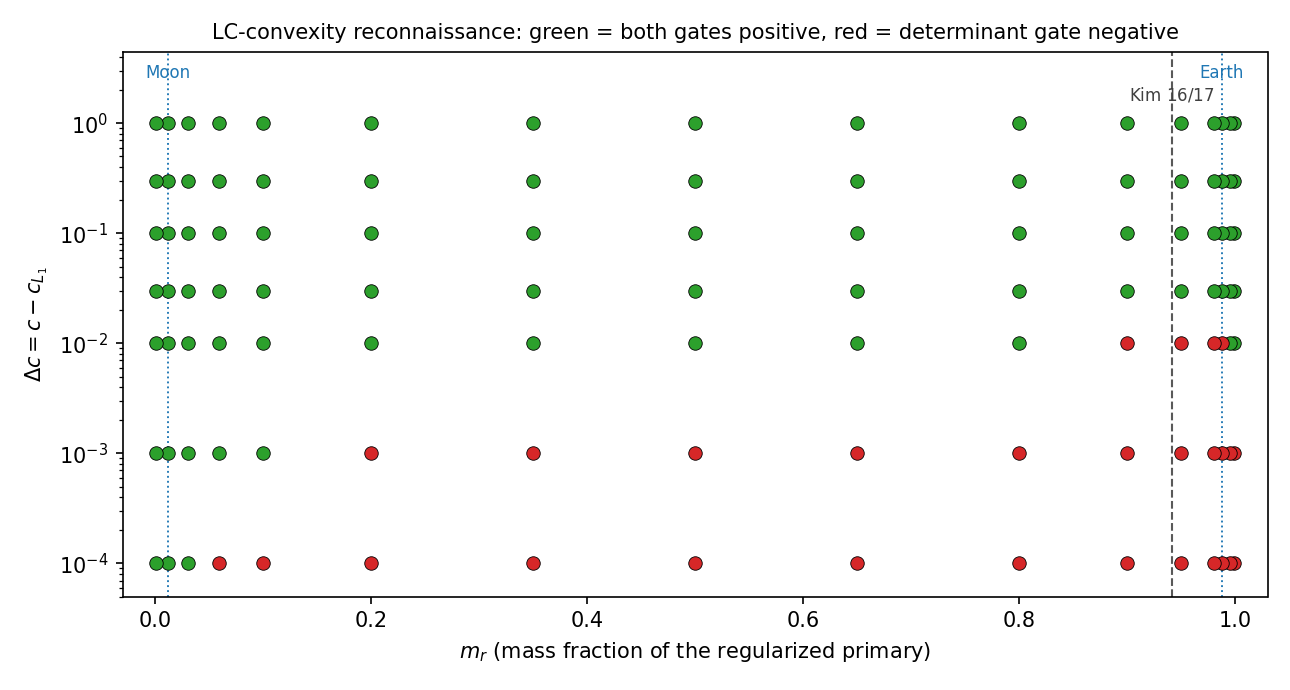
\includegraphics[width=0.86\textwidth]{figures/phase_map.png}
\caption{Floating-point reconnaissance of Levi--Civita convexity across the mass--energy plane, in the regularized-primary mass fraction $m_r$ (Remark~\ref{rem:mass}). Green markers: both reduced gates positive. Red markers: the determinant gate is negative (non-convex). Kim's $16/17$ threshold (his sufficient condition for near-critical non-convexity of the heavy component, $m_r<16/17$) and the Earth and Moon fractions are indicated. Near the critical energy the Moon component ($m_r\approx0.0122$) is convex while the Earth component ($m_r\approx0.9878$) is not; the critical limit $\Delta c\to 0^+$ is refined in Section~\ref{subsec:shell}.}
\label{fig:map}
\end{figure}

\subsection{Cross-check against Kim's threshold}
Kim~\cite[Thm.~1.3]{Kim} proves that the LC image of the regularized heavy-primary component is non-convex, for energies close to critical, once the heavy-primary mass fraction falls below $16/17=0.9412$. The corrected map is consistent with this sufficient condition: every heavy-side grid point with $m_r<16/17$ is indeed non-convex at $\Delta c=10^{-4}$. The map also shows that the condition is far from sharp near the critical energy: the non-convexity persists \emph{above} the threshold, through $m_r=0.95$, $0.98$, $0.995$ and $0.999$, with lobe depth decreasing toward the rotating-Kepler limit $m_r\to 1$. The light-side boundary of the window, located at $m_r\approx 0.045$ at $\Delta c=10^{-4}$, concerns the light component and is not covered by Kim's theorem. Version~1 of this paper claimed that the empirical boundary brackets $16/17$; as explained in the erratum note, that claim conflated the two conventions (the arithmetic coincidence $1-16/17=1/17$ placed the mislabeled light-side boundary near Kim's number) and is withdrawn.

\subsection{The Earth--Moon system}
The two components behave very differently. The Moon component ($m_r=0.0122$) lies below the light-side boundary and is LC-convex at every energy offset scanned in the map ($\Delta c\ge 10^{-4}$); this is the component of the certificate of Section~\ref{sec:earthmoon}, which operates at $\Delta c\approx 5.7\times10^{-3}$. The Earth component ($m_r=0.9878$), by contrast, sits inside the heavy-side window: it is non-convex at $\Delta c=10^{-4}$ with a macroscopic margin ($D_{\min}\approx-1.81$), and a dedicated energy sweep shows it recovers LC-convexity only at $\Delta c^{\mathrm E}\in(1.1\times10^{-2},\,1.2\times10^{-2})$ ($D_{\min}\approx-9.5\times10^{-3}$ at $\Delta c=1.1\times10^{-2}$ and $+1.1\times10^{-1}$ at $1.2\times10^{-2}$). The near-critical vicinity of the Moon component is refined next.

\subsection{Refinement at the critical limit: an ultrathin non-convex shell}\label{subsec:shell}
The map above has a smallest energy offset of $\Delta c=10^{-4}$. Refining the scan for the \emph{Moon} component ($m_r=0.012150585609624$, distant-primary parameter $\mu=0.987849414390376$, $c_{L_1}=1.594170558875$) down to $\Delta c=10^{-7}$, with a log-spaced energy grid, angular resolution up to $600$ base rays, $400$ radial samples, and the fiber minimum of $D$ evaluated on $1024$ angular samples of the exact degree-two polynomial of Lemma~\ref{lem:harm}, reveals a feature invisible at the coarser resolution: the true determinant minimum is \emph{negative} on an ultrathin shell immediately above the critical energy,
\[
c\in\bigl(c_{L_1},\,c_{L_1}+\Delta c^*\bigr],\qquad \Delta c^*\approx 9.54\times 10^{-6},
\]
the endpoint located by bisection in $\Delta c$. Three facts characterize the shell. First, the negativity is intrinsic to the critical limit and not a numerical artifact: as $\Delta c\to 0^+$ the determinant minimum converges monotonically to a strictly negative value ($D_{\min}\approx -1.5\times 10^{-6}$ at $\Delta c=10^{-6}$ and $\approx -1.7\times 10^{-6}$ at $\Delta c=10^{-7}$, the smallest offset probed), and the value is stable under refinement of the radial sampling ($n_s=60\to 400$) and of the fiber sampling ($512\to 1024$ angles). Second, the failure is again of the determinant only: the tangential surrogate $\calT$ remains strictly positive throughout the shell, so the surface is regular and develops a single saddle direction. Third, the minimizing base point sits at polar angle $\theta^*\approx 0.076$---essentially on the collision axis of the regularized primary---at $\approx 0.99$ of the boundary radius, far from the $s=\tfrac12$ singularity guard of the scan, ruling out a regularization artifact.

The mechanism is transparent: at $c=c_{L_1}$ the Lagrange point $L_1$ belongs to the energy hypersurface---the compact component touches the Hill neck---and the LC embedding degenerates there. This is the same mechanism underlying Kim's near-critical non-convexity theorem~\cite[Thm.~1.3]{Kim}, used in Section~\ref{sec:map} as a falsifiable cross-check; the quantitative content of the present refinement is that for the \emph{Moon} component of the Earth--Moon pair the phenomenon is confined to a shell of width $\sim 10^{-5}$ in $c$ rather than a macroscopic energy window. For the Earth component no analogous refinement is needed: it lies inside the macroscopic heavy-side window of the map, non-convex on the whole range $\Delta c\lesssim 1.2\times 10^{-2}$, so the shell phenomenon is subsumed there. (Version~1 attributed the shell to the Earth component and reported the Earth component's near-critical scan as convex; both statements followed from the convention error and the scanning heuristic, and are corrected here.)

Two consequences follow, both stated as numerical observations, and both now component-resolved. For the certification program, the LC-convexity route covers the Moon component for $c\ge c_{L_1}+10^{-5}$---essentially its entire subcritical regime---while the ultrathin shell $\bigl(c_{L_1},c_{L_1}+10^{-5}\bigr]$ and, more consequentially, the Earth component's macroscopic window $\bigl(c_{L_1},\,c_{L_1}+1.2\times10^{-2}\bigr)$ require the dynamical criterion (fiberwise convexity or nonnegativity of Conley--Zehnder indices, in the spirit of Kim's Theorem~1.4) rather than LC-convexity. For the interval certificate of Section~\ref{sec:earthmoon}, which concerns the Moon component at $\Delta c\in[5.73,5.93]\times 10^{-3}$---some six hundred times the shell width---nothing changes.

\section{A dynamical-relevance observation}\label{sec:relevance}

The non-convexity of Section~\ref{sec:map} is a property of the LC embedding, not directly of the dynamics. We record here a numerical observation---exploratory, floating-point---bearing on whether the non-convexity is dynamically relevant.

\begin{observation}\label{obs:abas}
Across the comparable-mass window (distant-primary parameter $\mu$ from $0.2$ to $0.6$, i.e.\ regularized fractions $m_r$ from $0.8$ down to $0.4$; energies just below critical), the region where the determinant gate is negative forms a pair of lateral lobes hugging the collar: in base polar coordinates the lobes occupy radial fraction $s/s^\ast\in[0.96,1.0]$ and angular band $\theta\in[3^\circ,12^\circ]$, displaced from both coordinate axes by at least $2^\circ$--$4^\circ$. Along the two axes, which carry the collision orbits, the true determinant minimum is strictly positive; for equal masses at $c=c_{L_1}+10^{-3}$ it is $+2.055\times10^{-1}$ along the retrograde axis and $+5.190$ along the direct axis.
\end{observation}

Figure~\ref{fig:relevance} displays the lobes and the determinant profile along the retrograde axis. In the LC model the retrograde periodic orbit of Birkhoff is the collision orbit along the axis joining the primaries~\cite{Kim}; Observation~\ref{obs:abas} says that this orbit, and its direct counterpart, traverse strictly convex portions of the surface, while the non-convexity sits laterally off-axis.

\begin{figure}[t]
\centering
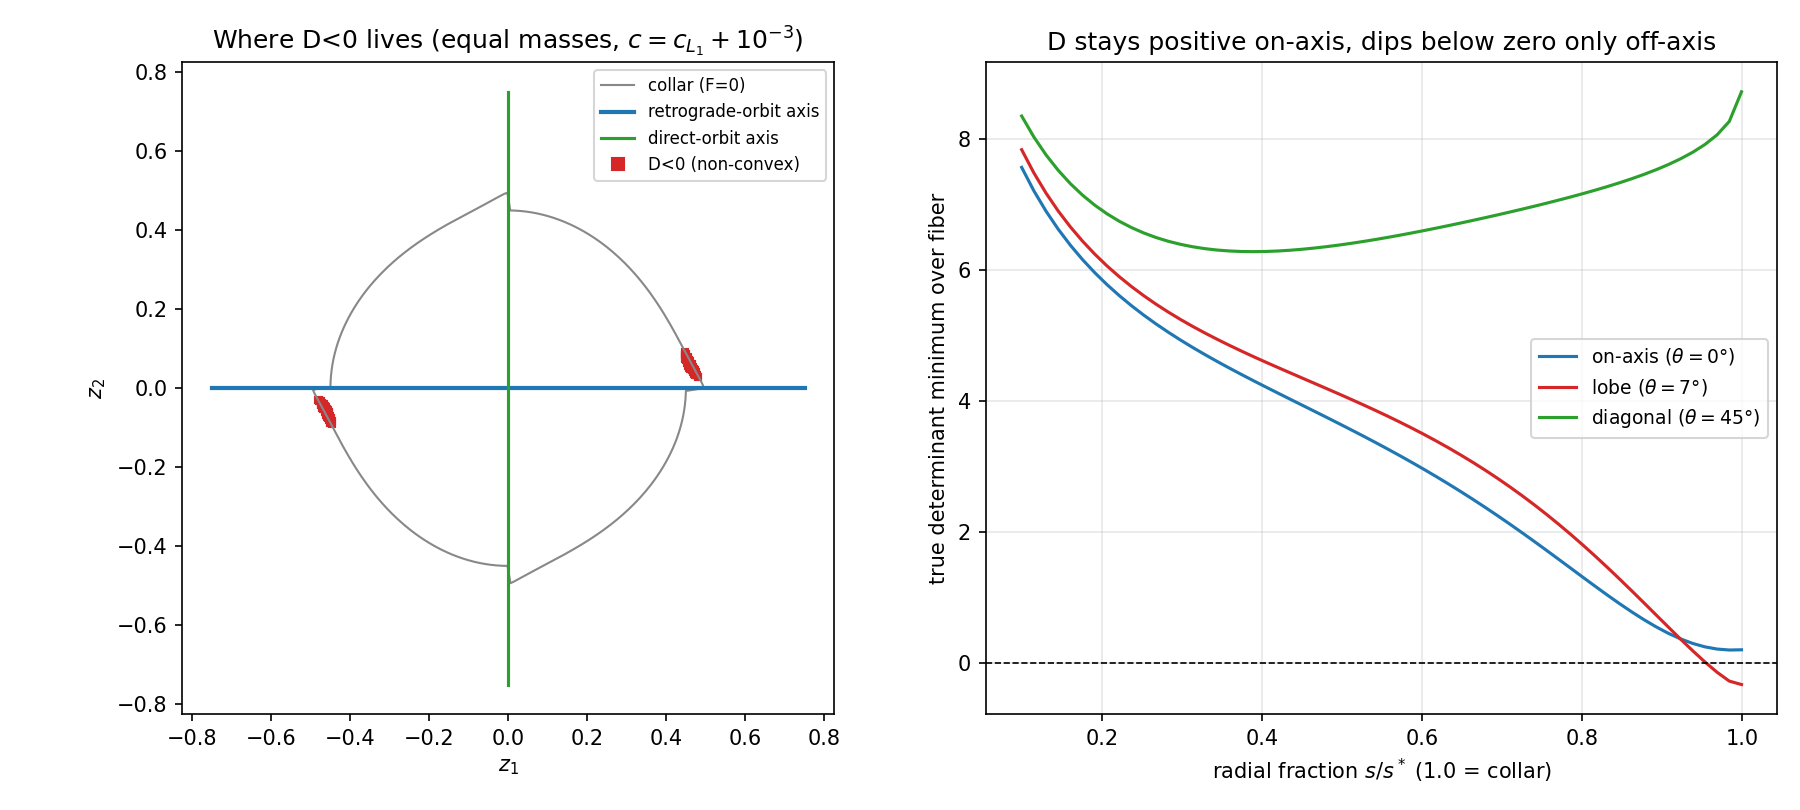
\includegraphics[width=\textwidth]{figures/dynamical_relevance.png}
\caption{Left: the non-convexity lobes (red) hug the collar off-axis; the retrograde-orbit axis passes between them. Right: the true determinant minimum along three rays---on-axis it stays positive to the collar; only the off-axis lobe dips below zero. Floating-point, equal masses, $c=c_{L_1}+10^{-3}$.}
\label{fig:relevance}
\end{figure}

We stress the limits of this observation. The hypothesis of~\cite{HS} is a condition on the Conley--Zehnder indices of \emph{all} closed Reeb orbits, not only the two collision orbits; a generic periodic orbit could still visit the lobes. Observation~\ref{obs:abas} is therefore evidence, not proof, that the non-convexity is dynamically inert, and it is floating-point at a finite grid. It does, however, delineate precisely where a rigorous analysis of the comparable-mass regime must concentrate.

\subsection{Fine structure of the lobes: a single simple fold}\label{subsec:fold}
A closer look at the lobes records two further numerical regularities, both stable across the comparable-mass band $\mu\in[0.2,0.8]$ (equivalently $m_r\in[0.2,0.8]$) at $c=c_{L_1}+10^{-3}$. They sharpen Observation~\ref{obs:abas} from ``$D$ becomes negative off-axis'' to a statement about \emph{how} it becomes negative.

\begin{observation}\label{obs:fold}
Throughout the lobes the reduced tangential gate $\mathcal T$ remains strictly positive, with a uniform margin: the minimum of $\mathcal T$ over the set $\{D<0\}$ decreases monotonically from $+7.5\times10^{-1}$ at $\mu=0.20$ to $+2.6\times10^{-1}$ at $\mu=0.80$, while $\min D$ over the same set rises from $-1.69$ to $-1.4\times10^{-3}$ as the lobes shrink. Consequently, at every lobe point the convexity pencil has $\operatorname{tr}>0$ and $\det<0$, hence exactly one negative principal direction: the LC non-convexity is a \emph{single simple fold}, never a double concavity.
\end{observation}

The two gates are precisely the trace and determinant data of the convexity pencil (Section~\ref{sec:gates}): $\mathcal T$ is the fiber-minimum of the trace gate and $D$ the fiber-minimum of the determinant gate. Where $D<0<\mathcal T$ the pencil is indefinite with a one-dimensional negative cone, the mildest possible failure of positive-definiteness. The fold is simple in the technical sense that the shape operator acquires a single negative eigenvalue on the lobe, not two; the saddle direction of Section~\ref{sec:map} is unique. Figure~\ref{fig:fold} shows the two gates along a lobe ray and their minima across the band.

\begin{figure}[t]
\centering
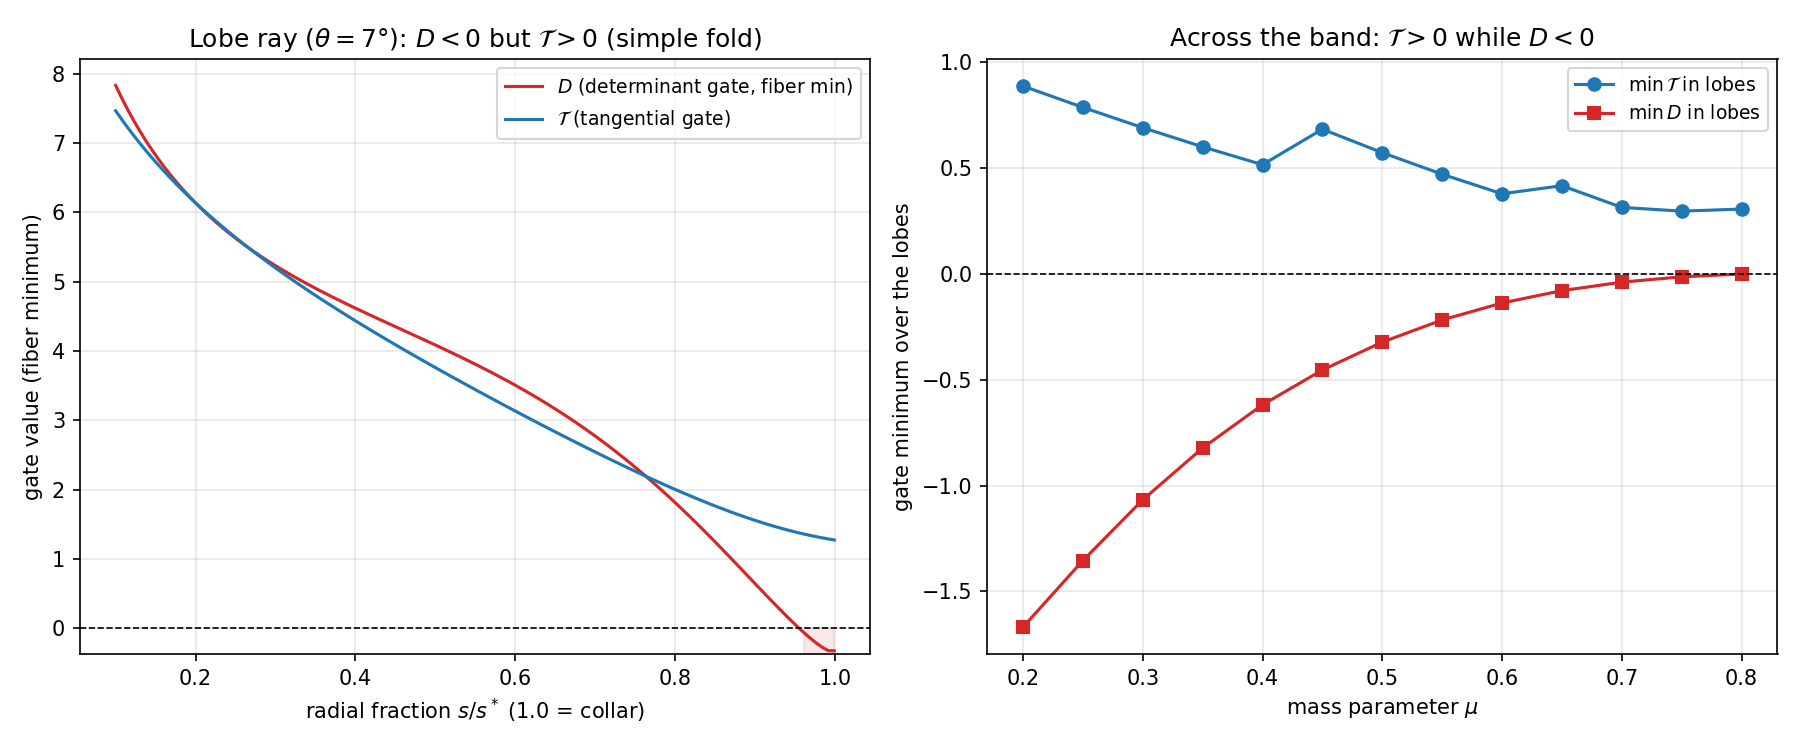
\includegraphics[width=\textwidth]{figures/lobe_structure.png}
\caption{Fine structure of the lobes (floating-point, $c=c_{L_1}+10^{-3}$). Left: along a lobe ray ($\theta=7^\circ$, equal masses) the determinant gate $D$ dips below zero near the collar while the tangential gate $\mathcal T$ stays strictly positive---a single simple fold. Right: across the comparable-mass band, $\min\mathcal T$ over the lobes stays uniformly positive while $\min D$ is negative, vanishing only as the lobes close near $\mu\to 0.8$.}
\label{fig:fold}
\end{figure}

A companion regularity concerns the radial geometry rather than the fiber. Along every ray the defining function $F$ crosses the collar transversally with $\partial F/\partial r<0$, uniformly (the collar radial derivative ranges from $-2.5\times10^{-1}$ at $\mu=0.20$ to $-1.0\times10^{-1}$ at $\mu=0.80$), on rays through the lobes no less than on-axis. Thus the bounded base component is radially star-shaped, and the LC non-convexity does not erode the star-shape margin: the surface that fails to be \emph{convex} on the lobes remains \emph{star-shaped} there, consistent with the general star-shapedness of the subcritical components~\cite{AFKP} and with the dynamical criterion of~\cite{HS} operating on star-shaped $S^3$. Both regularities are reproduced by \texttt{code/lobe\_structure.py} in the reproducibility package; like Observation~\ref{obs:abas} they are floating-point at a finite grid and are stated as such.

\section{Limitations and outlook}\label{sec:outlook}

The reduction of Section~\ref{sec:elimination} is exact and unconditional, and it makes the LC-convexity certificate substantially cheaper wherever LC-convexity holds---by the reconnaissance of Section~\ref{sec:map}: throughout the light-primary components ($m_r\lesssim 0.045$ near critical, including the Moon component of the Earth--Moon pair), and at energy offsets $\Delta c\gtrsim 0.03$ for every mass ratio (for the Earth component, $\Delta c\gtrsim 1.2\times 10^{-2}$). Two limitations bound its reach.

First, the reduced determinant gate uses the sufficient condition $\calD>0$, which is sharp only on the collar; away from the collar $\calD$ may be conservative, and a base point with $\calD<0<\min_\phi D$ would require the full harmonic minimum of Lemma~\ref{lem:harm} rather than the amplitude bound. This is a matter of tightness, not of correctness.

Second, and more fundamentally, the LC-convexity route is provably incapable of reaching the near-critical regime except for very light regularized primaries: by Kim's theorem~\cite[Thm.~1.3]{Kim} the LC embedding of the heavy component is non-convex there below the $16/17$ fraction, and the corrected reconnaissance of Section~\ref{sec:map} shows the offending window is in fact much larger, reaching essentially to the rotating-Kepler limit on the heavy side ($m_r$ up to $0.999$ at $\Delta c=10^{-4}$) and down to $m_r\approx 0.045$ on the light side. The refinement of Section~\ref{subsec:shell} shows that a residue of the same phenomenon persists even for the Moon component of the Earth--Moon pair, as an ultrathin non-convex shell of width $\approx 10^{-5}$ above the critical energy; and the Earth component is non-convex on the macroscopic window $\Delta c\lesssim 1.2\times 10^{-2}$. Any LC-based certification of the full subcritical range must therefore hand the near-critical regime to a dynamical argument. Two routes past this ceiling are natural. (i) A direct verification of dynamical convexity through the Conley--Zehnder indices of the closed orbits, which does not require convexity of any embedding but is computationally heavier; the simple-fold structure of Observation~\ref{obs:fold} localizes this analysis precisely, since only orbits entering the thin off-axis lobes can encounter the single negative principal direction, and the base there is still star-shaped. (ii) Kim's convex elliptic (two-center) embedding, proved for the Euler problem~\cite[Thm.~1.1]{Kim} and for small rotation strength~\cite[Rmk.~1.2]{Kim}, extended to the full rotating PCR3BP. Regarding the latter we record one exact fact that bears on its difficulty. In the doubly-covered elliptic coordinates $(\lambda,\nu)$ of~\cite{Kim}, the regularized rotation term is
\begin{equation}\label{eq:rotation}
(\cosh^2\lambda-\cos^2\nu)\,(q_1 p_2 - q_2 p_1) = \tfrac12\bigl(p_\lambda\sin 2\nu + p_\nu\sinh 2\lambda\bigr),
\end{equation}
a closed form that is \emph{linear in the momenta}. Consequently, for any rotation strength $a>0$ the regularized Hamiltonian $Q_c^a = Q^1(\lambda,p_\lambda) + Q^2(\nu,p_\nu) + a\cdot\tfrac12(p_\lambda\sin 2\nu + p_\nu\sinh 2\lambda)$ ceases to be mechanical, so the reduction of fiberwise convexity to planar-curve curvature that underlies Kim's proof (his Section~5, valid for the mechanical case $a=0$) no longer applies: a genuinely new argument, not a substitution into the Euler-problem proof, is required. Whether the off-axis lobes of Observation~\ref{obs:abas} are dynamically inert---so that the Birkhoff conjecture might hold in the comparable-mass regime despite the LC non-convexity---remains open, and is not settled by the evidence presented here.

\section*{Data and Code Availability}

The computational code developed for this study is publicly available on GitHub at \url{https://github.com/seu-usuario/seu-repositorio} (version 1.3.2, which implements the corrections described in the erratum note of Section~\ref{sec:map}; the file \texttt{ERRATUM.md} documents the changes, and \texttt{audit/audit\_artigo1.py} independently verifies both the mass convention of Remark~\ref{rem:mass} and the scanning-heuristic failure of version~1). The exact version used to generate the results presented here has been archived and is available on Zenodo under DOI \url{https://doi.org/10.5281/zenodo.XXXXXXX}.

\appendix

\section{The symbolic audit}\label{app:audit}

The following identities are checked by forming each residual and simplifying it to zero with a computer-algebra system. All eight residuals vanish identically; the driver prints \texttt{PASS\_C82\_FIBER\_ELIMINATION\_AUDIT}. The complete script is included in the reproducibility package as \texttt{code/fiber\_elimination\_audit.py}.

\begin{enumerate}
\item[R1] Gap formula~\eqref{eq:Tgap}: $T-\calT-64F^{3/2}(\sqrt s-z_2\cos\phi+z_1\sin\phi)=0$.
\item[R2] Perfect square~\eqref{eq:sq}: $s-(-z_2\cos\phi+z_1\sin\phi)^2-(z_1\cos\phi+z_2\sin\phi)^2=0$.
\item[R3] Attained angle: $\sqrt s-z_2(z_2/\sqrt s)+z_1(-z_1/\sqrt s)=0$.
\item[R4] Gradient reduction~\eqref{eq:grad}: $|\Fz|^2-(4sF_s^2+8aF_sF_a+4sF_a^2)=0$.
\item[R5] Laplacian reduction~\eqref{eq:lap}: $\Delta F-(4sF_{ss}+8aF_{sa}+4sF_{aa}+4F_s)=0$.
\item[R6] Generic harmonic decomposition~\eqref{eq:harm}: difference of the two sides $=0$ for arbitrary symmetric $L_0,M_1,M_2$, vector $g$, and scalars $\rho,F$.
\item[R7] Determinant sum~\eqref{eq:detsum}: $\det M_1+\det M_2-32s=0$.
\item[R8] Amplitude~\eqref{eq:detsum}: $(\det M_1-\det M_2)^2+\sigma(M_1,M_2)^2-(64s)^2=0$.
\end{enumerate}

Separately, the closed form~\eqref{eq:rotation} for the regularized rotation term in the doubly-covered elliptic coordinates, quoted in Section~\ref{sec:outlook}, is verified both symbolically (residual simplifies to $0$) and numerically (maximum deviation $<10^{-13}$ over $2\times10^5$ random points) by \texttt{code/rotation\_term\_audit.py}, which prints \texttt{PASS\_ROTATION\_TERM\_AUDIT}.

\begin{thebibliography}{10}

\bibitem{AFKP}
A.~Albers, U.~Frauenfelder, O.~van Koert, and G.~P.~Paternain,
\emph{Contact geometry of the restricted three-body problem},
Comm. Pure Appl. Math. \textbf{65} (2012), no.~2, 229--263.

\bibitem{Birkhoff}
G.~D.~Birkhoff,
\emph{The restricted problem of three bodies},
Rend. Circ. Mat. Palermo \textbf{39} (1915), 265--334.

\bibitem{GrisaCertificate}
C.~A.~Grisa,
\emph{A computer-assisted strict-convexity certificate near the Earth--Moon parameter and a Birkhoff global-section corollary},
companion manuscript (2026).

\bibitem{HWZ}
H.~Hofer, K.~Wysocki, and E.~Zehnder,
\emph{The dynamics on three-dimensional strictly convex energy surfaces},
Ann. of Math. (2) \textbf{148} (1998), no.~1, 197--289.

\bibitem{HS}
U.~L.~Hryniewicz and P.~A.~S.~Salom\~ao,
\emph{Global surfaces of section for dynamically convex Reeb flows on lens spaces},
Trans. Amer. Math. Soc. \textbf{368} (2016), 6403--6445.

\bibitem{Kim}
S.~Kim,
\emph{On a convex embedding of the Euler problem of two fixed centers},
arXiv:1701.07258 (2017).

\bibitem{LeviCivita}
T.~Levi-Civita,
\emph{Sur la r\'egularisation du probl\`eme des trois corps},
Acta Math. \textbf{42} (1920), 99--144.

\end{thebibliography}

\end{document}
